\chapter{Progettazione del database}
\label{cha:database}
I database vengono utilizzati per archiviare e manipolare grandi quantità di informazioni strutturate e non strutturate \cite{database}. L'approccio delle basi di dati racchiude alcune caratteristiche molto importanti, tra cui l'uso di strumenti per auto descrivere i dati collezionati memorizzandone la struttura (meta dati) e fornire la separazione tra programmi e informazioni, ottenendo il vantaggio di poter modificare l'uno o l'altro in maniera indipendente. Una base di dati permette anche di astrarre dai dettagli di memorizzazione dei dati, proponendo diverse rappresentazioni concettuali dei dati e garantisce l'elaborazione delle transizioni multiutente.\\
\newline
Il processo generale di design di un database prevede tre fasi principali:
\begin{enumerate}
    \item Progettazione concettuale
    \item Progettazione logica
    \item Progettazione fisica
\end{enumerate}
\noindent
La prima fase ha come scopo, lavorando sui requisiti raccolti, quello di produrre in output un modello concettuale, ovvero tradurre i problemi e le esigenze emerse in una mappatura semplice da comprendere e comunicare.
Questo tipo di progettazione prevede la definizione di entità (elementi base le cui proprietà sono descritte dagli attributi) e relazioni (che collegano due entità distinte con un particolare significato). L'obiettivo è quindi usare questi schemi (come i diagrammi ER o EER) per semplificare la gestione del database e, al contempo, poter comunicare la struttura generale dei dati richiesta in modo astratto.
La fase successiva serve invece a produrre lo schema logico, partendo da quello appena creato, usando indici e chiavi esterne per definire in modo formale le relazioni tra i dati e ottenere una rappresentazione astratta di una possibile implementazione non vincolata ad alcuna tecnologia specifica. Il modello logico più usato in questo stadio dello sviluppo è quello relazionale. La progettazione fisica, infine, produce lo schema interno della base di dati, in termini di scelta del DBMS (Database Management System) \cite{dbms}, strutture di memorizzazione delle tabelle, organizzazione dei file e dei permessi utente.
\begin{figure}[!hbt]
\centering

\includegraphics[scale=0.50]{img/desing_db.png}
\caption{Processo di progettazione di un database}
\label{fig:design_db}
\end{figure}
\noindent

\section{Tecnologie utilizzate}
\label{sec:dbtech}
Per la corretta gestione e inserimento dei dati, grazie anche all'analisi dei requisiti, è stato progettato il database su cui il sistema appoggia usando come RDBMS (Relational database management system) il servizio MySQL \cite{mysql} in quanto semplice da gestire, gratuito, veloce e, soprattutto, estremamente compatibile con PHP. Per amministrare e configurare il database è stato usato phpMyAdmin \cite{phpmyadmin} mentre per la creazione e modellazione della base di dati si è scelto come strumento MySQL Workbench \cite{mysqlworkbench}.

\section{Diagramma EER}
\label{sec:db}
Un diagramma EER (Extended or Enhanced Entity-Relationship) \cite{eer} è un tipo di schema concettuale che fornisce una rappresentazione visiva della struttura del database sia in fase di creazione, che a processo completo. Oltre agli elementi concettuali di base presenti negli schemi ER tradizionali questo modello aggiunge concetti più sofisticati come sottoclassi e super classi, specializzazioni e generalizzazioni, categorie ed ereditarietà di attributi e relazioni. \\
\newline
In figura \ref{fig:DiagrammaEER} viene mostrato il diagramma EER completo usato per la progettazione del database.
\begin{figure}[!hbt]
\centering
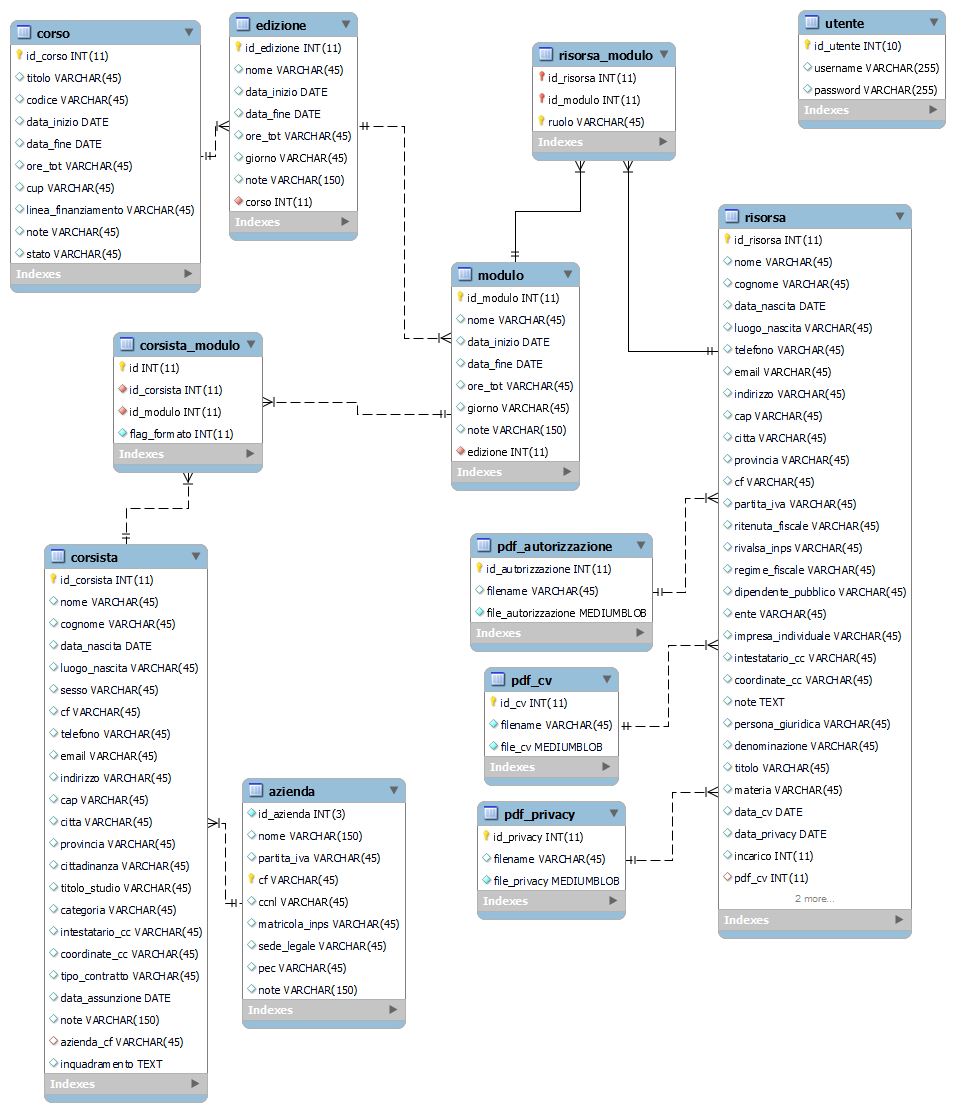
\includegraphics[scale=0.50]{img/EER.png}
\caption{Diagramma EER del database}
\label{fig:DiagrammaEER}
\end{figure}

\section{Normalizzazione e forme normali}
\label{sec:normalizzazione}
Una tecnica usata per la verifica dei risultati della progettazione di una base di dati è la normalizzazione, che consiste nel trasformare schemi non normalizzati in schemi che soddisfano una forma normale. Lo scopo è quindi passare per ogni relazione, da una con ridondanze a una assente di difetti, il che è sinonimo di qualità. Le anomalie delle relazioni possono essere risolte seguendo le forme normali, in particolare la Prima Forma Normale (1NF) richiede che tutti gli attributi dello schema non siano composti o multi valore; vale invece la Seconda Forma Normale (2NF) se, oltre a essere in 1NF, ogni attributo non appartenente a nessuna chiave dipende completamente da ogni chiave (quindi non dipende da una parte di chiave). I requisiti della Terza forma normale (3NF) sono che, oltre a valere la 2NF, tutti gli attributi non chiave devono dipendere direttamente dalla chiave, quindi non possono esserci attributi dipendenti da altri attributi che non sono presenti in chiave. La Forma Normale di Boyce-Codd (BCNF) prevede, di fatto, che ogni attributo dal quale ne dipendono altri possa svolgere la funzione di chiave, oltre a essere in 1NF.\\
\newline
Per quanto riguarda il modello elaborato per il progetto, la Prima Forma Normale è già parte integrante della definizione formale di relazione nel modello relazionale. Non essendoci dipendenze parziali tra attributi dalle varie chiavi, anche la Seconda Forma Normale è rispettata. Non vale invece la 3 NF in quanto esistono dipendenze tra le colonne di una tabella basate su attributi che non sono chiave primaria; ad esempio nella tabella \verb|corsista| è presente il campo \verb|data_assunzione| che non è subordinato alla chiave primaria della tabella. Sono perciò presenti attributi non chiave che dipendono transitivamente dalla chiave. Il livello di normalizzazione usato è quindi quello di 2NF. Uno dei presupposti per un futuro rilascio del sistema potrebbe essere quello di arrivare a rispettare la Terza forma normale adattando di conseguenza le relazioni della base di dati.



\section{Traduzione in SQL}
Durante la fase di progettazione logica, SQL (Structured Query Language) è il linguaggio usato dai modelli relazionali per permettere le operazioni di creazione o modifica dello schema (DDL: Data Definition Language) e di interrogazione, inserimento, modifica o eliminazione dei dati (DML: Data Manipulation Language). A titolo di esempio si riporta il codice in SQL per la creazione della tabella \verb|modulo| della base di dati (listing \ref{code:sql}).

\begin{listing}[h]
\begin{minted}{SQL}
CREATE TABLE `modulo` (
  `id_modulo` int(11) NOT NULL,
  `nome` varchar(45) DEFAULT NULL,
  `data_inizio` date DEFAULT NULL,
  `data_fine` date DEFAULT NULL,
  `ore_tot` varchar(45) DEFAULT NULL,
  `giorno` varchar(45) DEFAULT NULL,
  `note` varchar(150) DEFAULT NULL,
  `edizione` int(11) NOT NULL
) ENGINE=InnoDB DEFAULT CHARSET=utf8mb4;
-- Indici per le tabelle `modulo`
ALTER TABLE `modulo`
  ADD PRIMARY KEY (`id_modulo`),
  ADD KEY `fk_modulo_edizione1` (`edizione`);
-- Limiti per la tabella `modulo`
ALTER TABLE `modulo`
  ADD CONSTRAINT `fk_modulo_edizione1` FOREIGN KEY
  (`edizione`) REFERENCES `edizione` (`id_edizione`)
  ON DELETE NO ACTION ON UPDATE NO ACTION;
\end{minted}
\caption{codice SQL per la creazione della tabella \textit{Modulo}}
\label{code:sql}
\end{listing}


\clearpage
\newpage
